\documentclass[brazil]{article}
\usepackage[T1]{fontenc}
\usepackage[utf8x]{inputenc}
\usepackage[a4paper]{geometry}
\geometry{verbose,tmargin=1.2cm,bmargin=1.5cm,lmargin=1.5cm,rmargin=1.5cm}
\usepackage{calc}
\usepackage{amsthm}
\usepackage{amsmath}
\usepackage{float}
\usepackage{graphicx}
\usepackage{setspace}
\usepackage{babel}


%\usepackage{eso-pic}
%\newcommand\BackgroundPic{
%\put(0,0){
%\parbox[b][\paperheight]{\paperwidth}{%
%\vfill
%\centering
%
\includegraphics[width=\paperwidth,height=\paperheight,keepaspectratio]{figs/UNIFOR_WM1.eps}
%\vfill
%}}}

\title{Física II / Lista 01}
\date{2014.2}
\author{Prof. Roberto Lima \\Universidade de Fortaleza}

\begin{document}
%\AddToShipoutPicture{\BackgroundPic} %INICIA MARCA D'AGUA
\maketitle

\begin{enumerate}

\item Um pião gira com aceleração angular $\alpha = 5t^3 - 4t$, onde $t$ está em segundos e $\alpha$ em radianos por segundo ao quadrado. No instante $t=0$, a velocidade angular do pião é $5\;\mbox{rad/s}$ e uma reta de referência traçada no pião está na posição angular $\theta=2\;\mbox{rad}$.
\begin{enumerate}
\item Obtenha uma expressão para a velocidade angular do pião, $\omega(t)$, ou seja, escreva uma expressão que descreva explicitamente a variação da velocidade angular com o tempo.
\item Obtenha uma expressão para a posição angular do pião, $\theta(t)$.
\end{enumerate}


\item Uma pedra de amolar (figura) gira com aceleração angular constante $\alpha=0,35\; rad/s^2$. No instante $t=0$, a pedra tem uma velocidade angular $\omega_0 = - 4,6\; rad/s$ e uma reta de referência traçada na pedra está na horizontal, na posição angular $\theta_0 = 0$.
\begin{figure}[H]
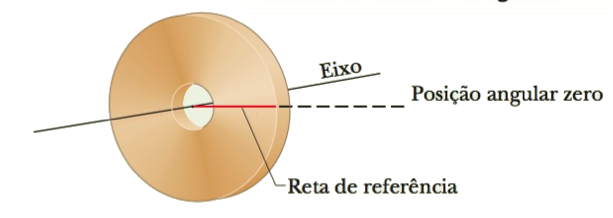
\includegraphics[scale=0.4]{figs/pedra-amolar.png}
\end{figure}
\begin{enumerate}
\item Em que instante após $t=0$ a reta de referência está na posição angular $\theta=5,0\;rev$?
\item Descreva a rotação da pedra de amolar entre $t=0$ e $t=32\;s$.
\item Em que instante $t$ a pedra de amolar para momentaneamente?
\end{enumerate}


\item Você está operando um rotor (um brinquedo de parque de diversões com um cilindro giratório vertical), percebe que um ocupaste está ficando tonto e reduz a velocidade angular do cilindro de $3,40\;rad/s$ para $2,00\;rad/s$ em $20,0\;rev$, com aceleração angular constante.
\begin{enumerate}
\item Qual é a aceleração angular constante durante esta redução de velocidade angular?
\item Em quanto tempo ocorre a redução de velocidade?
\end{enumerate}


\item A figura mostra um corpo rígido composto por duas partículas de massa ``m'' ligadas por uma barra de comprimento $L$ e massa desprezível.
\begin{figure}[H]
\hfill
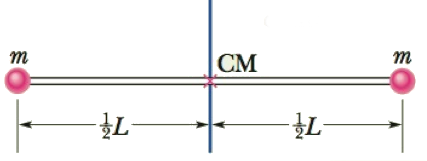
\includegraphics[scale=0.4]{figs/duas-particulas01.png}\hfill
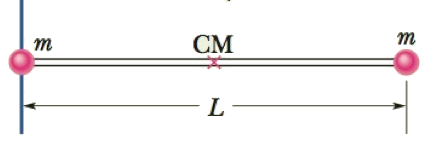
\includegraphics[scale=0.4]{figs/duas-particulas02.png}
\end{figure}
\begin{enumerate}
\item Qual o momento de inércia $I_{CM}$ em relação a um eixo passando pelo centro de massa e perpendicular à barra, como mostra a figura?
\item Qual o momento de inércia $I$ do corpo em relação a um eixo passando pela extremidade esquerda da barra e paralelo ao primeiro eixo (fig b)?
\end{enumerate}


\item A figura mostra uma barra fina, homogênea, de massa $M$ e comprimento $L$, e um eixo $x$ ao longo da barra cuja origem coincide com o centro da barra.
\begin{figure}[H]
\hfill 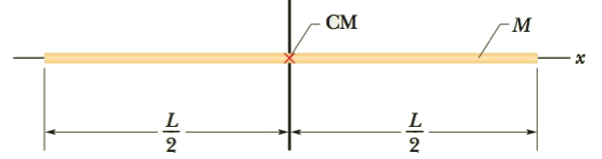
\includegraphics[scale=0.4]{figs/barra-momento.png}
\end{figure}
\begin{enumerate}
\item Qual o momento de inércia da barra em relação à um eixo perpendicular à barra passando pelo centro.
\item Qual o momento de inércia $I$ da barra em relação a um novo eixo perpendicular à barra passando pela extremidade esquerda?
\end{enumerate}


\item Em um teste foi utilizado um rotor maciço de aço, forma de disco, com uma massa de $M=272\;kg$ em um raio $R=38,0\;cm$. Quando atingiu uma velocidade angular de $14.000\;rev/min$, houve uma explosão. O chão de concreto abaixo da câmara tinha afundado $0,5\;cm$ e a tampa de $900\;kg$ tinha sido lançada para cima, atravessando o teto e caíra de volta, destruindo o equipamento. Qual a energia liberada na explosão do rotor?


\item A figura mostra um disco homogêneo, de massa $M=2,5\;kg$ e raio $R=20\;cm$, montado em um eixo horizontal fixo. Um bloco de massa $m=1,2\;kg$ está pendurado por uma corda de massa desprezível enrolada na borda do disco. Determine a aceleração do bloco em queda, a aceleração angular do disco e a tensão na corda. A corda não escorrega e não existe atrito no eixo.
\begin{figure}[H]
\hfill 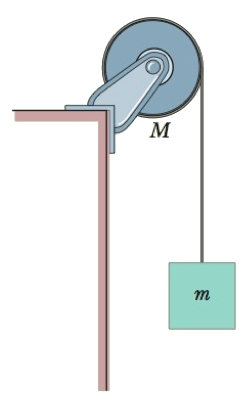
\includegraphics[scale=0.4]{figs/disco-homogeneo.png}
\end{figure}
	

\item Uma bola homogênea, de massa $M=6,00\;kg$ de raio $R$, rola suavemente a partir do repouso, descendo uma rampa inclinada de ângulo $\theta=30,0^{\circ}$.
\begin{enumerate}
\item A bola desce uma distância vertical $h=1,20\;m$ para chegar à base da rampa. Qual a velocidade da bola ao chegar à base da rampa?
\item Quais são o módulo e a orientação da força de atrito que age sobre a bola quando desce a rampa rolando?
\end{enumerate}
\begin{figure}[H]
\hfill 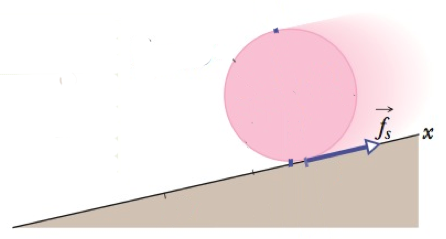
\includegraphics[scale=0.5]{figs/plano-inclinado01-mod.png}
\end{figure}


\end{enumerate}
\end{document}
